\nonstopmode
\documentclass[aspectratio=169,xcolor={svgnames}]{beamer}
\usepackage[utf8]{inputenc}
% \usepackage[frenchb]{babel}
\usepackage{amsmath}
\usepackage{mathtools}
\usepackage{breqn}
\usepackage{multirow}
\usetheme{boxes}
\usepackage{graphicx}
\usepackage{import}
\usepackage{adjustbox}
\usepackage[absolute,overlay]{textpos}
%\useoutertheme[footline=authortitle,subsection=false]{miniframes}
%\useoutertheme[footline=authorinstitute,subsection=false]{miniframes}
\useoutertheme{infolines}
\setbeamertemplate{headline}{}

\beamertemplatenavigationsymbolsempty

\definecolor{TitleOrange}{RGB}{255,137,0}
\setbeamercolor{title}{fg=TitleOrange}
\setbeamercolor{frametitle}{fg=TitleOrange}

\definecolor{ListOrange}{RGB}{255,145,5}
\setbeamertemplate{itemize item}{\color{ListOrange}$\blacktriangleright$}

\definecolor{verygrey}{RGB}{70,70,70}
\setbeamercolor{normal text}{fg=verygrey}


\usepackage{tabu}
\usepackage{multicol}
\usepackage{vwcol}
\usepackage{stmaryrd}
\usepackage{graphicx}

\usepackage[normalem]{ulem}

\AtBeginSection[]{
  \begin{frame}
  \vfill
  \centering
  \begin{beamercolorbox}[sep=8pt,center,shadow=true,rounded=true]{title}
    \usebeamerfont{title}\insertsectionhead\par%
  \end{beamercolorbox}
  \vfill
  \end{frame}
}

\title{Garage}
\author{Alex Auvolat, Deuxfleurs}
\date{Capitoul, 2024-02-29}

\begin{document}

\begin{frame}
	\centering
	
\includegraphics[width=.3\linewidth]{../../sticker/Garage.png}
	\vspace{1em}

	{\large\bf Alex Auvolat, Deuxfleurs Association}
	\vspace{1em}

	\url{https://garagehq.deuxfleurs.fr/}

	Matrix channel: \texttt{\#garage:deuxfleurs.fr}
\end{frame}

\begin{frame}
	\frametitle{Who I am}
	\begin{columns}[t]
		\begin{column}{.2\textwidth}
			\centering
			\adjincludegraphics[width=.4\linewidth, valign=t]{../assets/alex.jpg}
		\end{column}
		\begin{column}{.6\textwidth}
			\textbf{Alex Auvolat}\\
			PhD; co-founder of Deuxfleurs
		\end{column}
		\begin{column}{.2\textwidth}
			~
		\end{column}
	\end{columns}
	\vspace{2em}

	\begin{columns}[t]
		\begin{column}{.2\textwidth}
			\centering
			\adjincludegraphics[width=.5\linewidth, valign=t]{../assets/logos/deuxfleurs.pdf}
		\end{column}
		\begin{column}{.6\textwidth}
			\textbf{Deuxfleurs}\\
			A non-profit self-hosting collective,\\
			member of the CHATONS network
		\end{column}
		\begin{column}{.2\textwidth}
			\centering
			\adjincludegraphics[width=.7\linewidth, valign=t]{../assets/logos/logo_chatons.png}
		\end{column}
	\end{columns}

\end{frame}

\begin{frame}
	\frametitle{Our objective at Deuxfleurs}
	
	\begin{center}
		\textbf{Promote self-hosting and small-scale hosting\\
			as an alternative to large cloud providers}
	\end{center}
	\vspace{2em}
	\visible<2->{
		Why is it hard?
		\vspace{2em}
		\begin{center}
			\textbf{\underline{Resilience}}\\
			{\footnotesize we want good uptime/availability with low supervision}
		\end{center}
	}
\end{frame}

\begin{frame}
	\frametitle{Our very low-tech infrastructure}

	\only<1,3-6>{
		\begin{itemize}
			\item \textcolor<4->{gray}{Commodity hardware (e.g. old desktop PCs)\\
				\vspace{.5em}
				\visible<3->{{\footnotesize (can die at any time)}}}
				\vspace{1.5em}
			\item<4-> \textcolor<6->{gray}{Regular Internet (e.g. FTTB, FTTH) and power grid connections\\
				\vspace{.5em}
				\visible<5->{{\footnotesize (can be unavailable randomly)}}}
				\vspace{1.5em}
			\item<6-> \textbf{Geographical redundancy} (multi-site replication)
		\end{itemize}
	}
	\only<2>{
		\begin{center}
			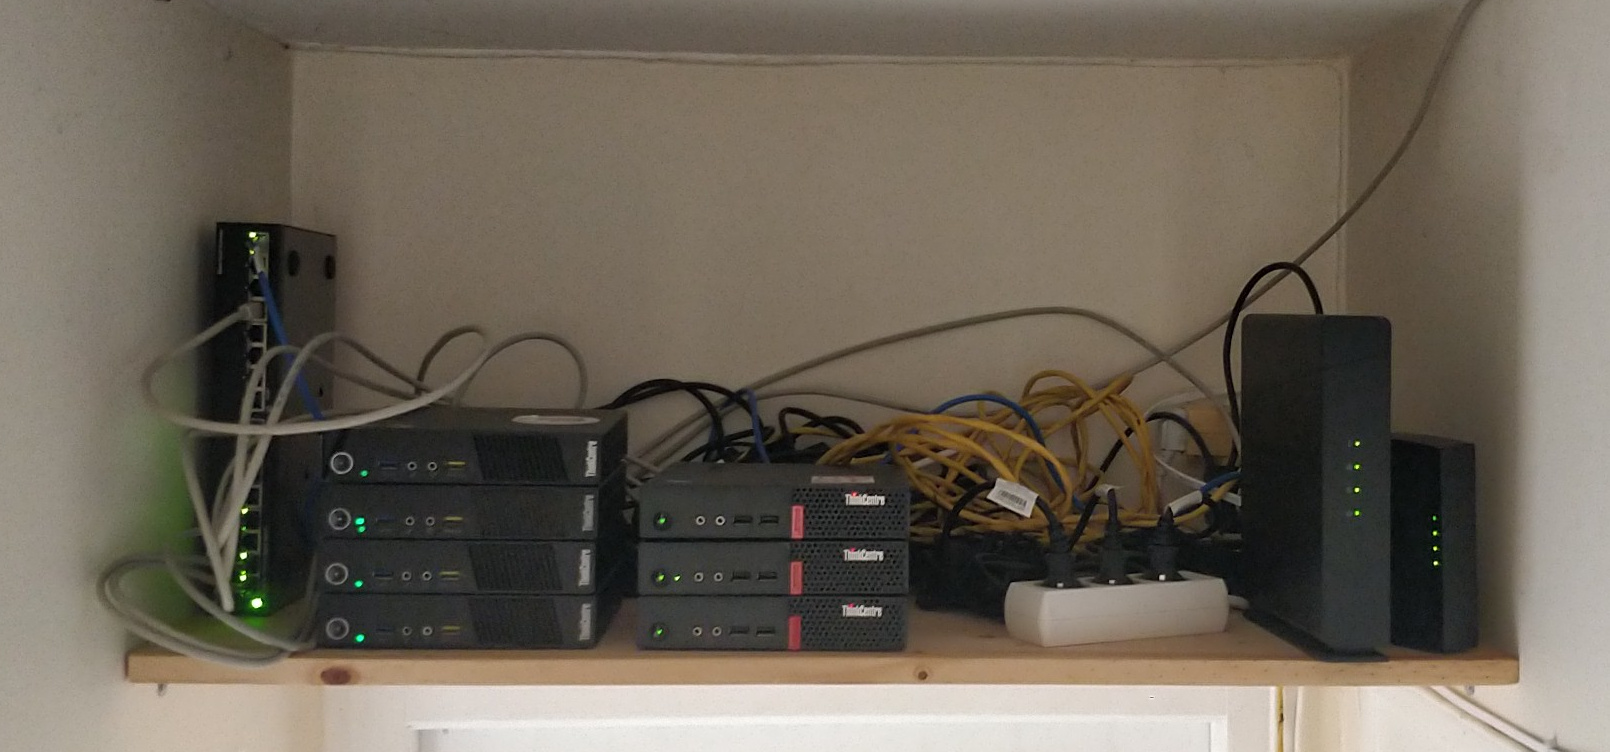
\includegraphics[width=.8\linewidth]{../assets/neptune.jpg}
		\end{center}
	}
	\only<7>{
		\begin{center}
			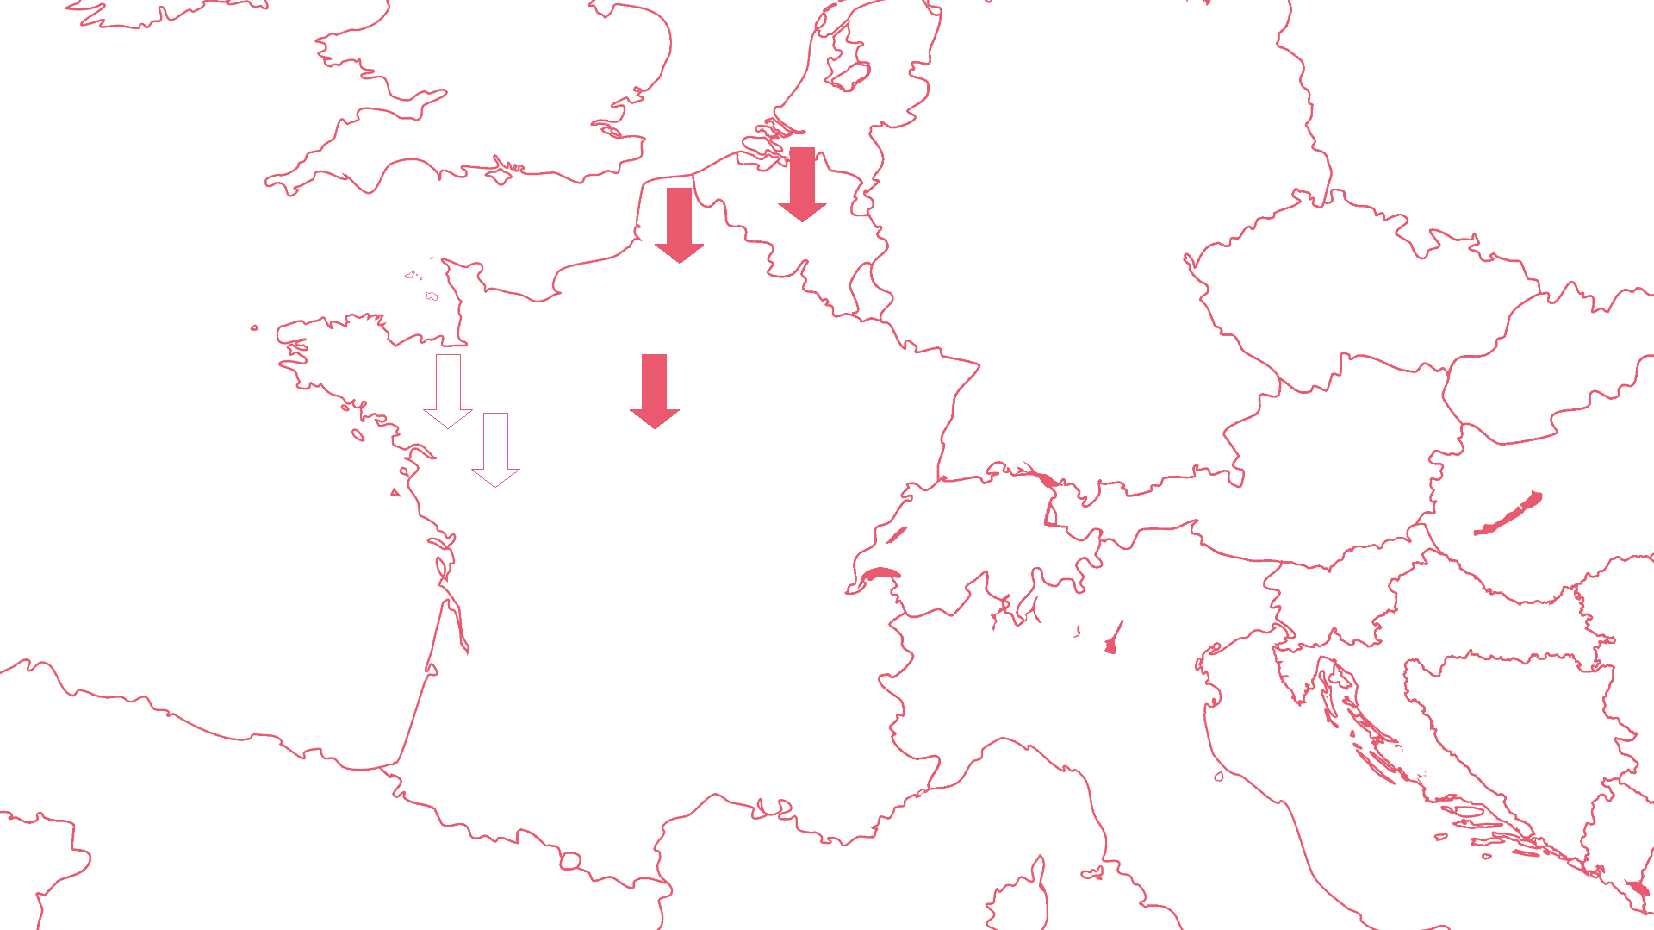
\includegraphics[width=.8\linewidth]{../assets/inframap_jdll2023.pdf}
		\end{center}
	}
\end{frame}

\begin{frame}
	\frametitle{How to make this happen}
	\begin{center}
		\only<1>{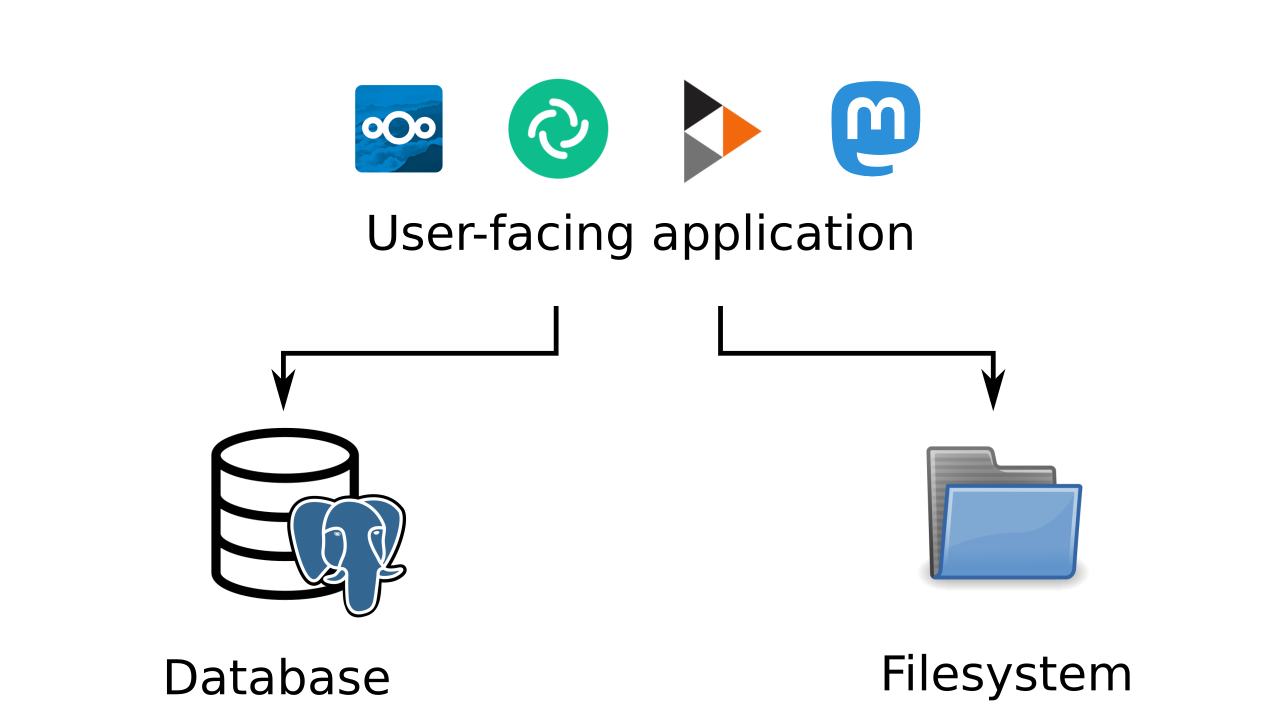
\includegraphics[width=.8\linewidth]{../assets/intro/slide1.png}}%
		\only<2>{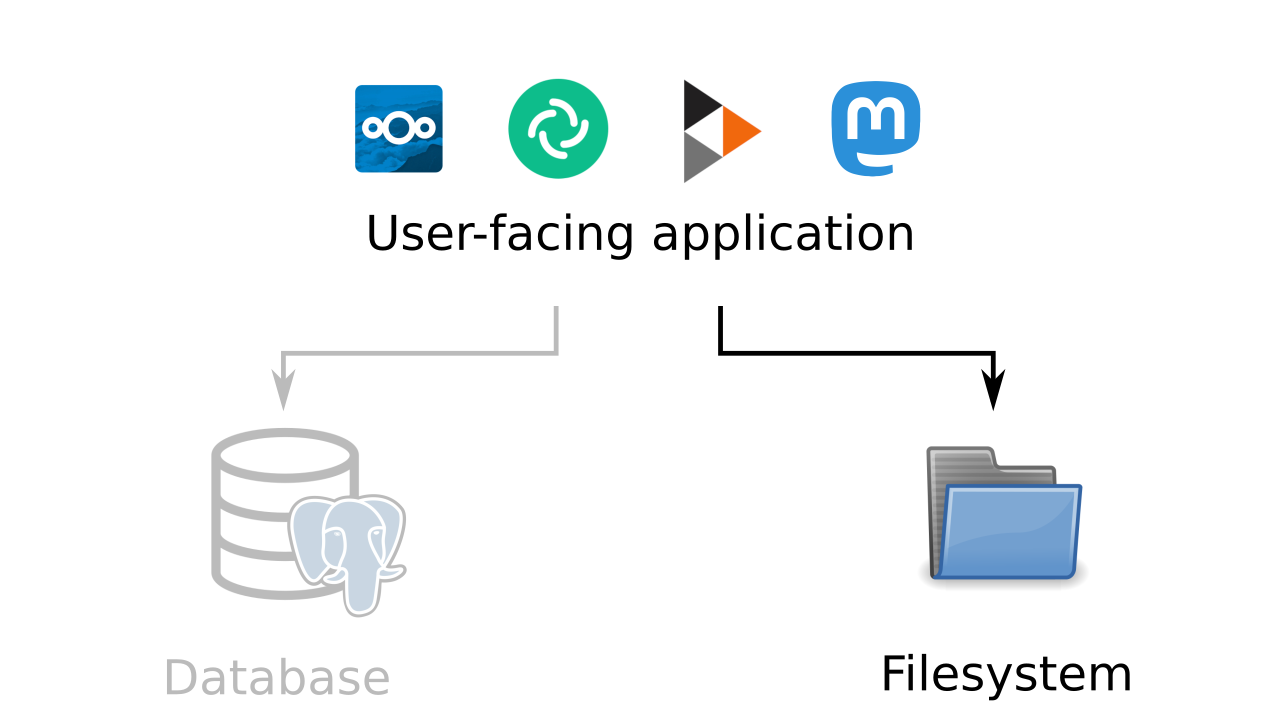
\includegraphics[width=.8\linewidth]{../assets/intro/slide2.png}}%
		\only<3>{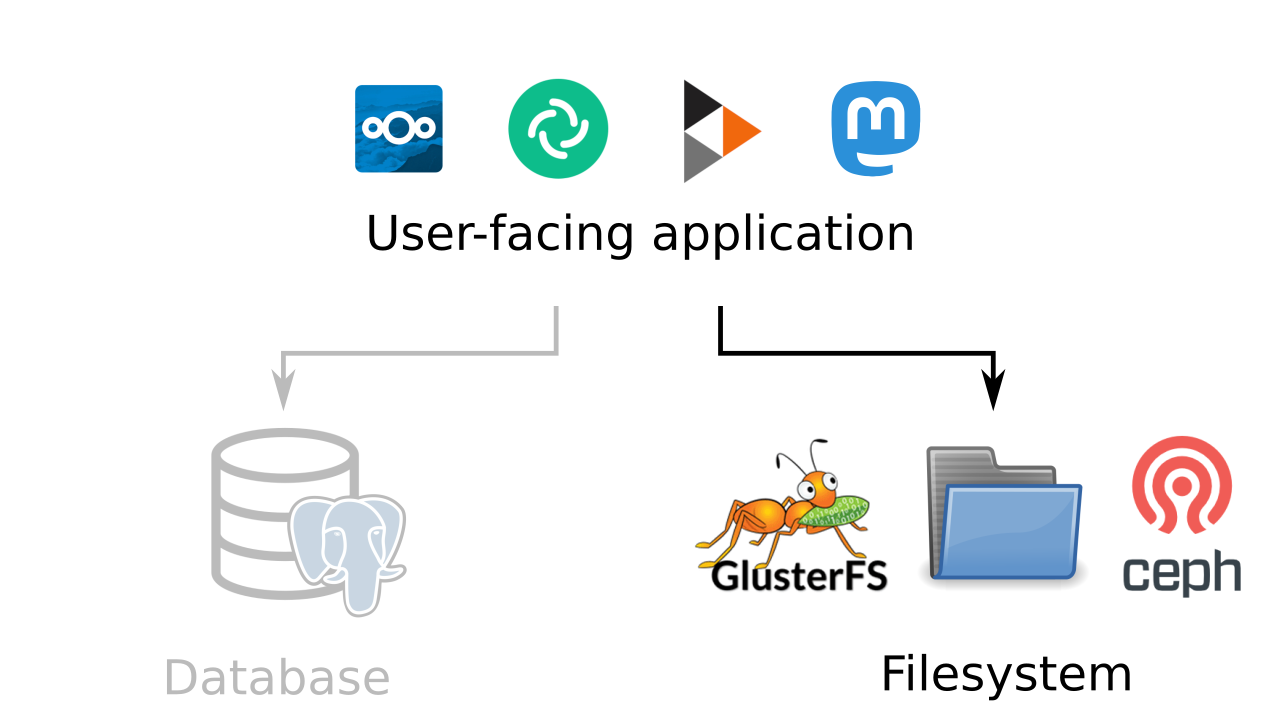
\includegraphics[width=.8\linewidth]{../assets/intro/slide3.png}}%
	\end{center}
\end{frame}

\begin{frame}
	\frametitle{Distributed file systems are slow}
	File systems are complex, for example:
	\vspace{1em}
	\begin{itemize}
		\item Concurrent modification by several processes
			\vspace{1em}
		\item Folder hierarchies
			\vspace{1em}
		\item Other requirements of the POSIX spec (e.g.~locks)
	\end{itemize}
	\vspace{1em}
	Coordination in a distributed system is costly

	\vspace{1em}
	Costs explode with commodity hardware / Internet connections\\
	{\small (we experienced this!)}
\end{frame}

\begin{frame}
	\frametitle{A simpler solution: object storage}
	Only two operations:
	\vspace{1em}
	\begin{itemize}
		\item Put an object at a key
			\vspace{1em}
		\item Retrieve an object from its key
	\end{itemize}
	\vspace{1em}
	{\footnotesize (and a few others)}

	\vspace{1em}
	Sufficient for many applications!
\end{frame}

\begin{frame}
	\frametitle{A simpler solution: object storage}
		\begin{center}
			
\includegraphics[height=6em]{../assets/logos/Amazon-S3.jpg}
			\hspace{3em}
			\visible<2->{
\includegraphics[height=5em]{../assets/logos/minio.png}}
			\hspace{3em}
			\visible<3>{
\includegraphics[height=6em]{../../logo/garage_hires_crop.png}}
		\end{center}
		\vspace{1em}
	S3: a de-facto standard, many compatible applications

	\vspace{1em}
	\visible<2->{MinIO is self-hostable but not suited for geo-distributed deployments}

	\vspace{1em}
	\visible<3->{\textbf{Garage is a self-hosted drop-in replacement for the Amazon S3 object store}}
\end{frame}

% --------- BASED ON CRDTS ----------

\section{Principle 1: based on CRDTs}

\begin{frame}
	\frametitle{CRDTs / weak consistency instead of consensus}

	\underline{Internally, Garage uses only CRDTs} (conflict-free replicated data types)

	\vspace{2em}
	Why not Raft, Paxos, ...? Issues of consensus algorithms:

	\vspace{1em}
	\begin{itemize}
		\item<2-> \textbf{Software complexity}
			\vspace{1em}
		\item<3-> \textbf{Performance issues:}
			\vspace{.5em}
			\begin{itemize}
				\item<4-> The leader is a \textbf{bottleneck} for all requests\\
					\vspace{.5em}
				\item<5-> \textbf{Sensitive to higher latency} between nodes
					\vspace{.5em}
				\item<6-> \textbf{Takes time to reconverge} when disrupted (e.g. node going down)
			\end{itemize}
	\end{itemize}
\end{frame}

\begin{frame}
	\frametitle{The data model of object storage}
	Object storage is basically a \textbf{key-value store}:
	\vspace{.5em}

	{\scriptsize
		\begin{center}
		\begin{tabular}{|l|p{7cm}|}
			\hline
			\textbf{Key: file path + name} & \textbf{Value: file data + metadata} \\
			\hline
			\hline
			\texttt{index.html} &
				\texttt{Content-Type: text/html; charset=utf-8} \newline
				\texttt{Content-Length: 24929} \newline
				\texttt{<binary blob>} \\ 
			\hline
			\texttt{img/logo.svg} &
				\texttt{Content-Type: text/svg+xml} \newline
				\texttt{Content-Length: 13429} \newline
				\texttt{<binary blob>} \\ 
			\hline
			\texttt{download/index.html} &
				\texttt{Content-Type: text/html; charset=utf-8} \newline
				\texttt{Content-Length: 26563} \newline
				\texttt{<binary blob>} \\ 
			\hline
		\end{tabular}
		\end{center}
		}

	\vspace{.5em}
	\begin{itemize}
		\item<2-> Maps well to CRDT data types
		\item<3> Read-after-write consistency with quorums
	\end{itemize}
\end{frame}


\begin{frame}
	\frametitle{Performance gains in practice}
	\begin{center}
		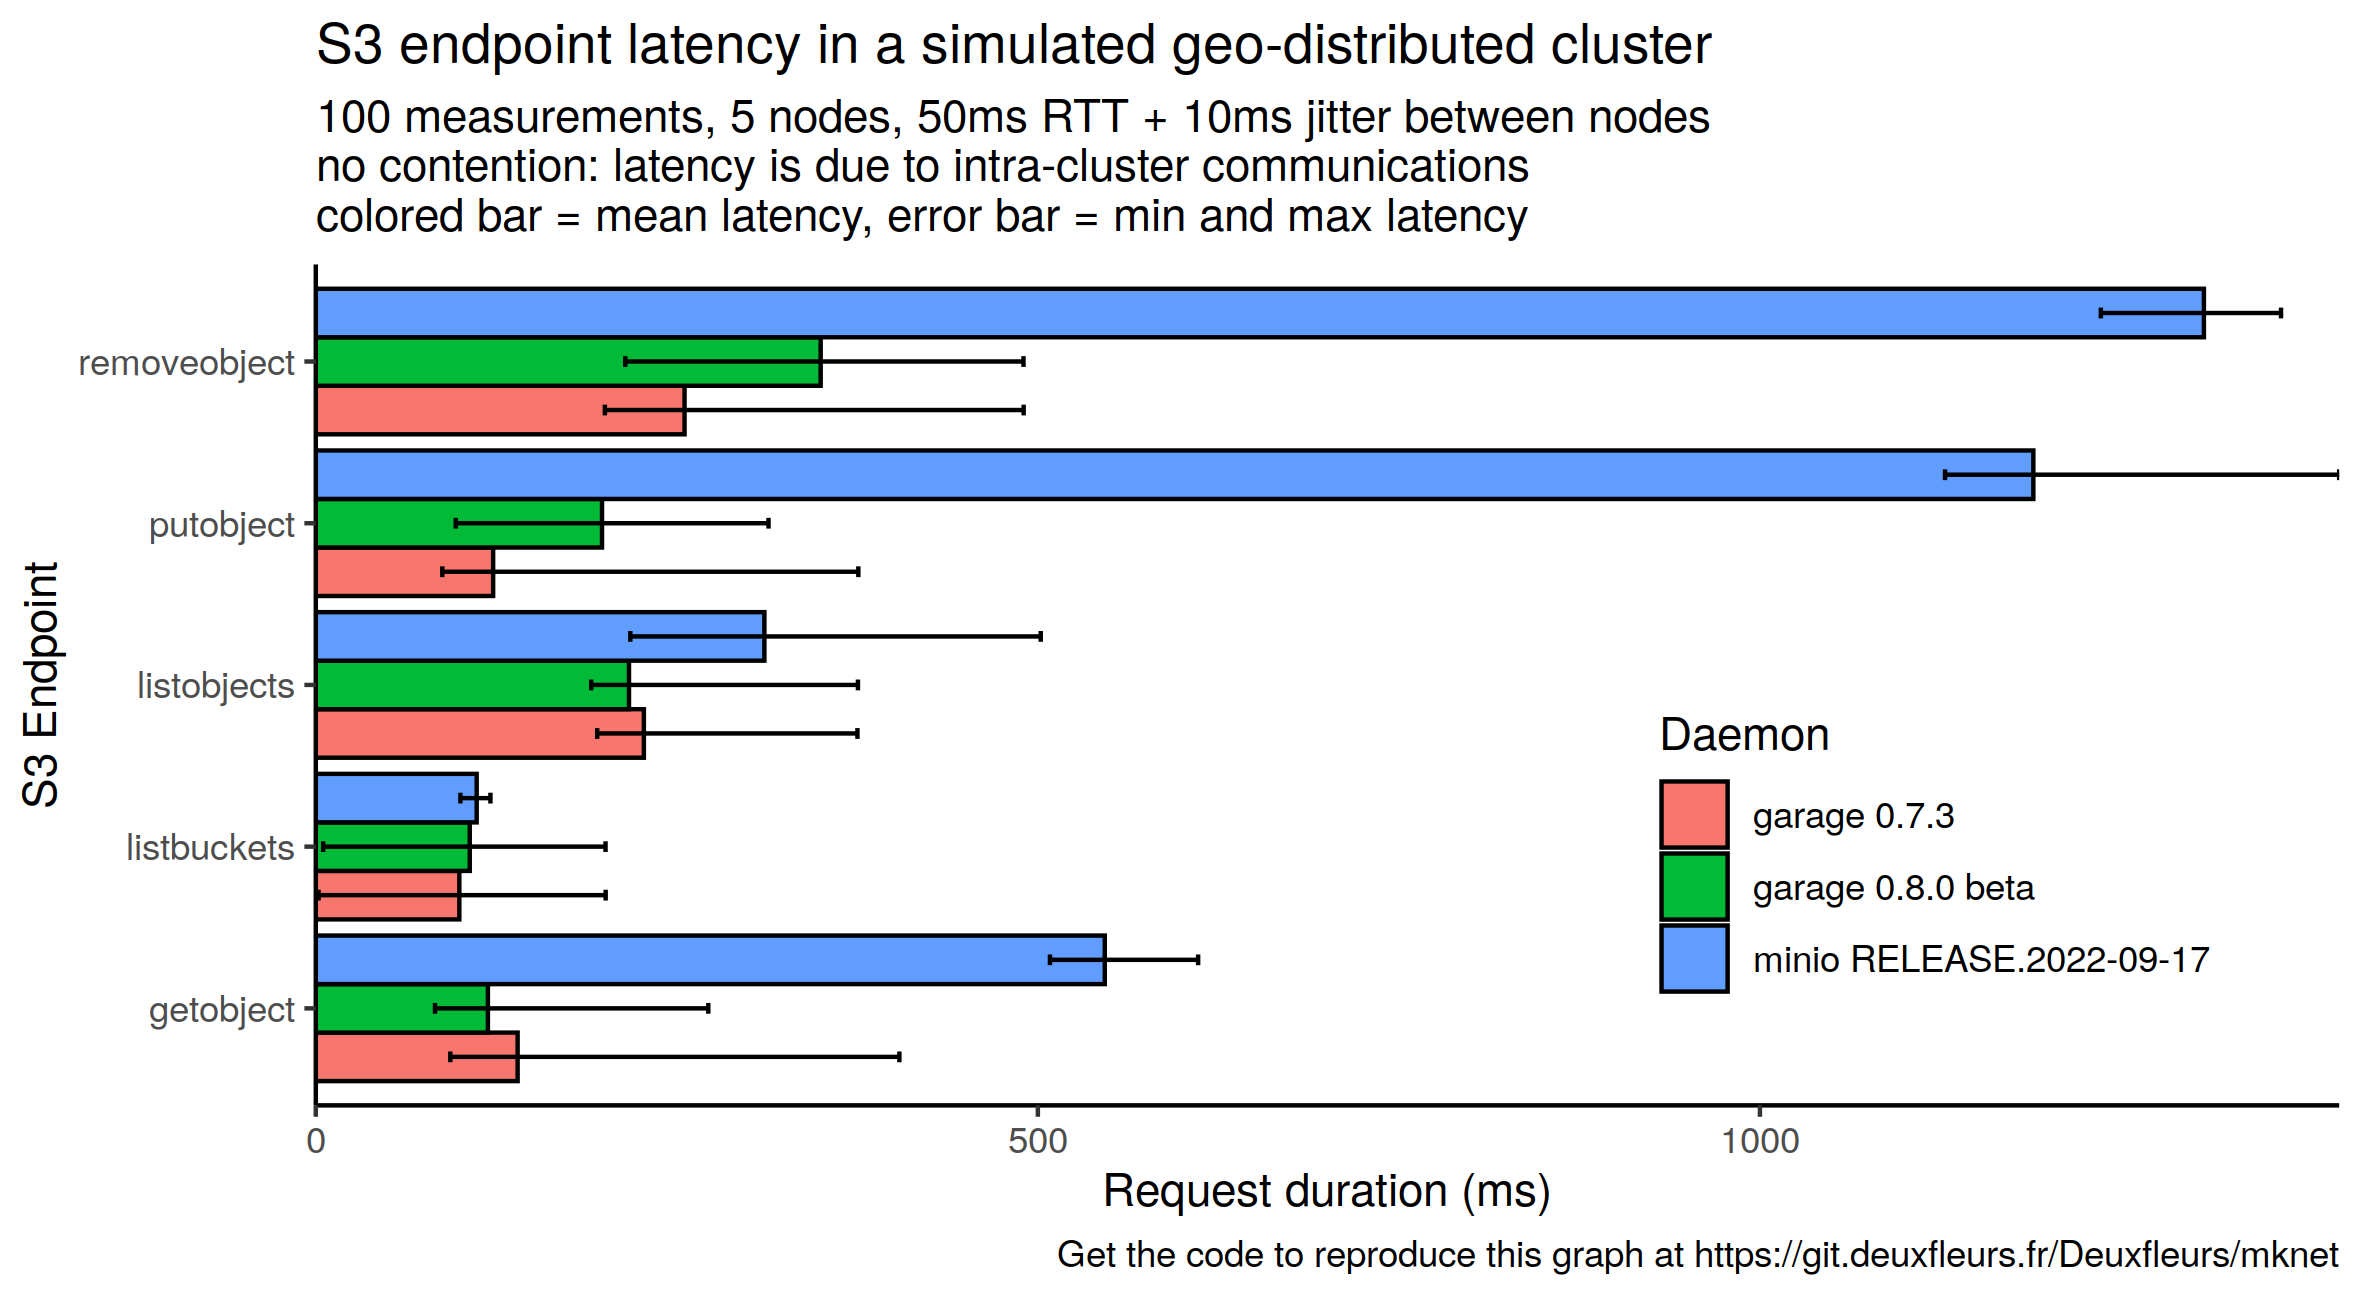
\includegraphics[width=.8\linewidth]{../assets/perf/endpoint_latency_0.7_0.8_minio.png}
	\end{center}
\end{frame}

% --------- GEO-DISTRIBUTED MODEL ----------

\section{Principle 2: geo-distributed data model}

\begin{frame}
	\frametitle{Key-value stores, upgraded: the Dynamo model}
	\textbf{Two keys:}
	\begin{itemize}
		\item Partition key: used to divide data into partitions {\small (a.k.a.~shards)}
		\item Sort key: used to identify items inside a partition
	\end{itemize}

	\vspace{1em}

	\begin{center}
	\begin{tabular}{|l|l|p{3cm}|}
		\hline
		\textbf{Partition key: bucket} & \textbf{Sort key: filename} & \textbf{Value} \\
		\hline
		\hline
		\texttt{website} & \texttt{index.html} & (file data) \\
		\hline
		\texttt{website} & \texttt{img/logo.svg} & (file data) \\
		\hline
		\texttt{website} & \texttt{download/index.html} & (file data) \\
		\hline
		\hline
		\texttt{backup} & \texttt{borg/index.2822} & (file data) \\
		\hline
		\texttt{backup} & \texttt{borg/data/2/2329} & (file data) \\
		\hline
		\texttt{backup} & \texttt{borg/data/2/2680} & (file data) \\
		\hline
		\hline
		\texttt{private} & \texttt{qq3a2nbe1qjq0ebbvo6ocsp6co} & (file data) \\
		\hline
	\end{tabular}
	\end{center}
\end{frame}


\begin{frame}
	\frametitle{Layout computation}
	\begin{overprint}
		\onslide<1>
		\begin{center}
			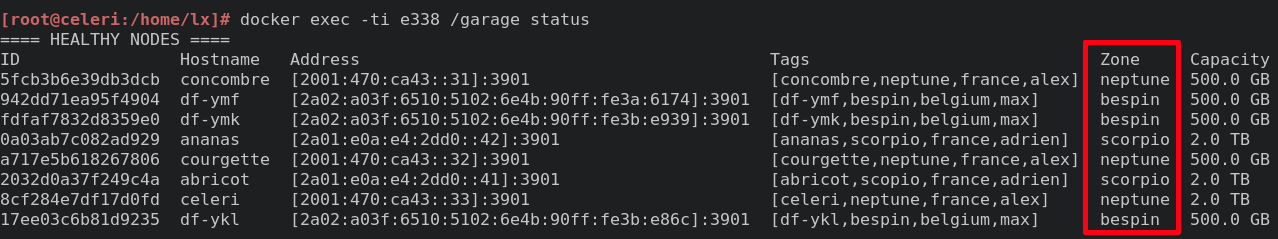
\includegraphics[width=\linewidth, trim=0 0 0 -4cm]{../assets/screenshots/garage_status_0.9_prod_zonehl.png}
		\end{center}
		\onslide<2>
		\begin{center}
			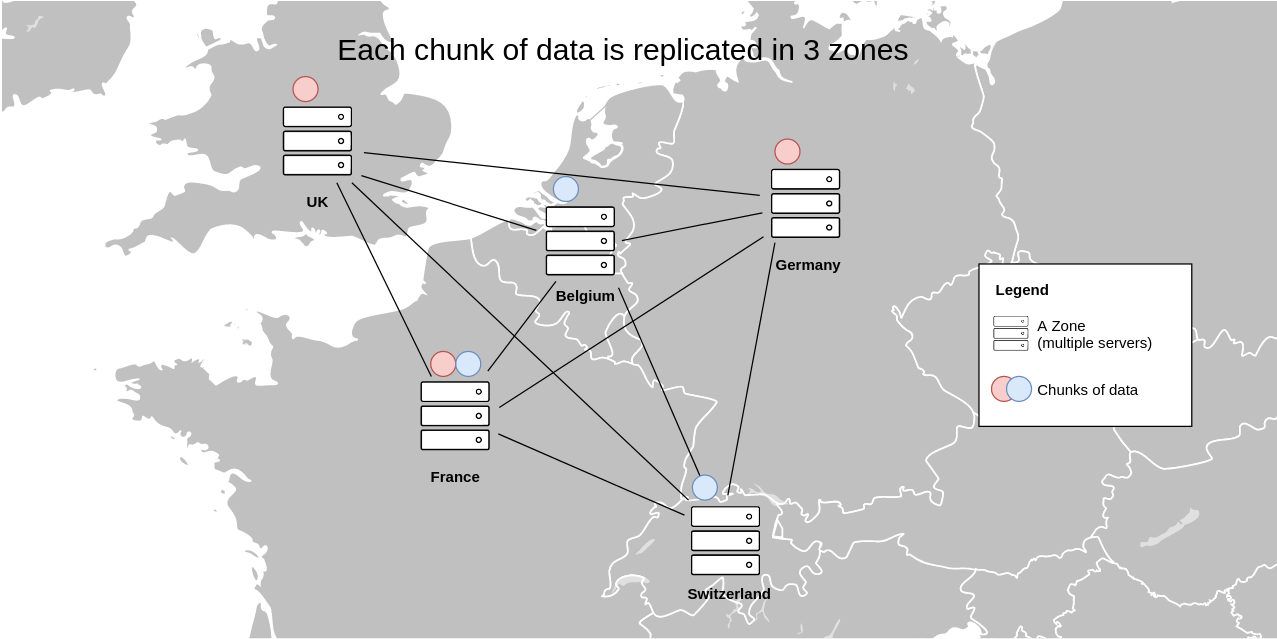
\includegraphics[width=.7\linewidth]{../assets/map.png}
		\end{center}
	\end{overprint}
	\vspace{1em}
	Garage stores replicas on different zones when possible
\end{frame}

\begin{frame}
	\frametitle{What a "layout" is}
		\textbf{A layout is a precomputed index table:}
		\vspace{1em}

		{\footnotesize
			\begin{center}
			\begin{tabular}{|l|l|l|l|}
				\hline
				\textbf{Partition} & \textbf{Node 1} & \textbf{Node 2} & \textbf{Node 3} \\
				\hline
				\hline
				Partition 0 & df-ymk (bespin) & Abricot (scorpio) & Courgette (neptune) \\
				\hline
				Partition 1 & Ananas (scorpio) & Courgette (neptune) & df-ykl (bespin) \\
				\hline
				Partition 2 & df-ymf (bespin) & Celeri (neptune) & Abricot (scorpio) \\
				\hline
				\hspace{1em}$\vdots$ & \hspace{1em}$\vdots$ & \hspace{1em}$\vdots$ & \hspace{1em}$\vdots$ \\
				\hline
				Partition 255 & Concombre (neptune) & df-ykl (bespin) & Abricot (scorpio) \\
				\hline
			\end{tabular}
			\end{center}
		}

	\vspace{2em}
	\visible<2->{
		The index table is built centrally using an optimal algorithm,\\
		then propagated to all nodes
	}

	\vspace{1em}
	\visible<3->{
		\footnotesize
		Oulamara, M., \& Auvolat, A. (2023). \emph{An algorithm for geo-distributed and redundant storage in Garage}.\\ arXiv preprint arXiv:2302.13798.
	}
\end{frame}


\begin{frame}
	\frametitle{The relationship between \emph{partition} and \emph{partition key}}
	\begin{center}
	\begin{tabular}{|l|l|l|l|}
		\hline
		\textbf{Partition key} & \textbf{Partition} & \textbf{Sort key} & \textbf{Value} \\
		\hline
		\hline
		\texttt{website} & Partition 12 & \texttt{index.html} & (file data) \\
		\hline
		\texttt{website} & Partition 12 & \texttt{img/logo.svg} & (file data) \\
		\hline
		\texttt{website} & Partition 12 &\texttt{download/index.html} & (file data) \\
		\hline
		\hline
		\texttt{backup} & Partition 42 & \texttt{borg/index.2822} & (file data) \\
		\hline
		\texttt{backup} & Partition 42 & \texttt{borg/data/2/2329} & (file data) \\
		\hline
		\texttt{backup} & Partition 42 & \texttt{borg/data/2/2680} & (file data) \\
		\hline
		\hline
		\texttt{private} & Partition 42 & \texttt{qq3a2nbe1qjq0ebbvo6ocsp6co} & (file data) \\
		\hline
	\end{tabular}
	\end{center}
	\vspace{1em}
	\textbf{To read or write an item:} hash partition key
	\\ \hspace{5cm} $\to$ determine partition number (first 8 bits)
	\\ \hspace{5cm} $\to$ find associated nodes
\end{frame}

\begin{frame}
	\frametitle{Garage's internal data structures}
	\centering
	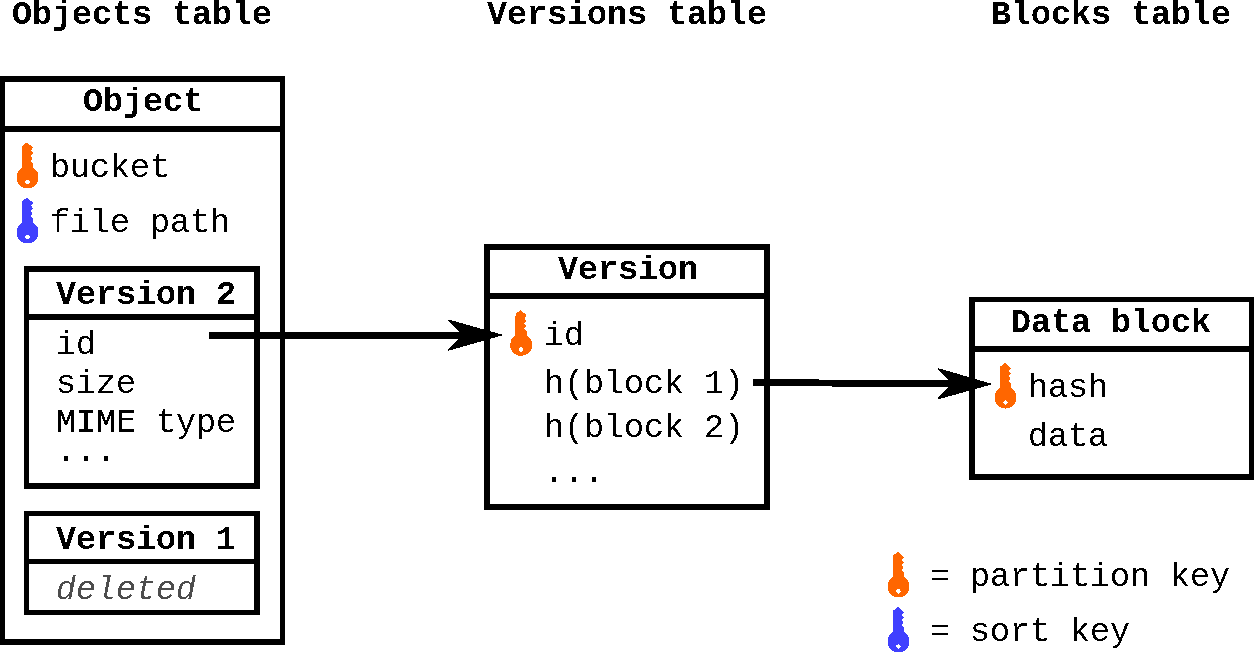
\includegraphics[width=.75\columnwidth]{../assets/garage_tables.pdf}
\end{frame}

% ---------- OPERATING GARAGE ---------

\section{Operating Garage clusters}

\begin{frame}
	\frametitle{Operating Garage}
	\begin{center}
		\only<1-2>{
			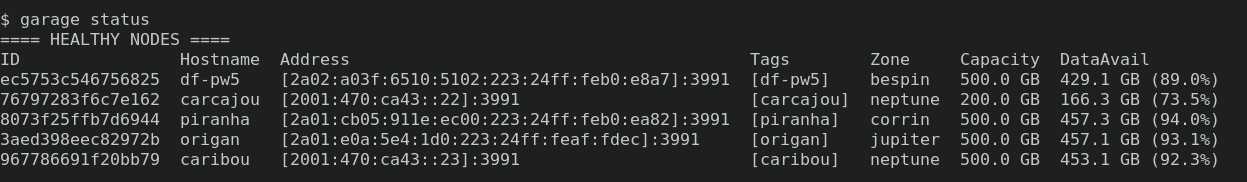
\includegraphics[width=.9\linewidth]{../assets/screenshots/garage_status_0.10.png}
			\\\vspace{1em}
			\visible<2>{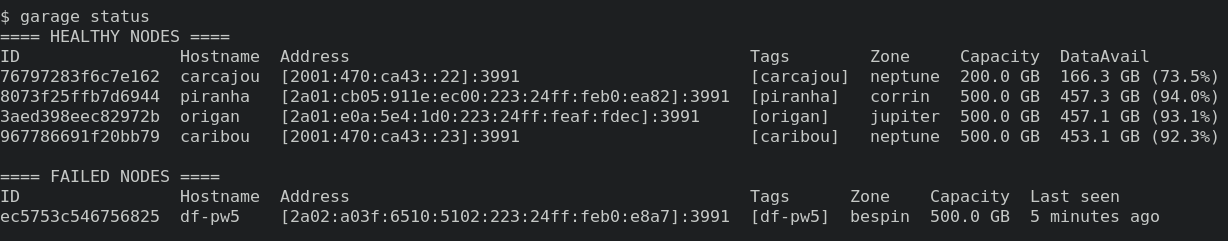
\includegraphics[width=.9\linewidth]{../assets/screenshots/garage_status_unhealthy_0.10.png}}
		}
	\end{center}
\end{frame}

\begin{frame}
	\frametitle{Background synchronization}
	\begin{center}
		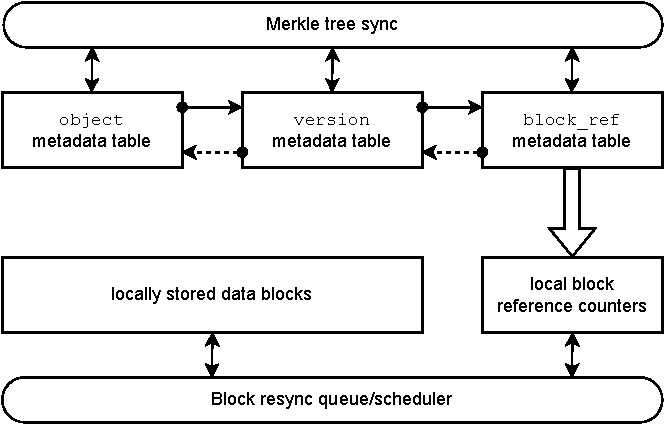
\includegraphics[width=.6\linewidth]{../assets/garage_sync.drawio.pdf}
	\end{center}
\end{frame}

\begin{frame}
	\frametitle{Digging deeper}
	\begin{center}
		\only<1>{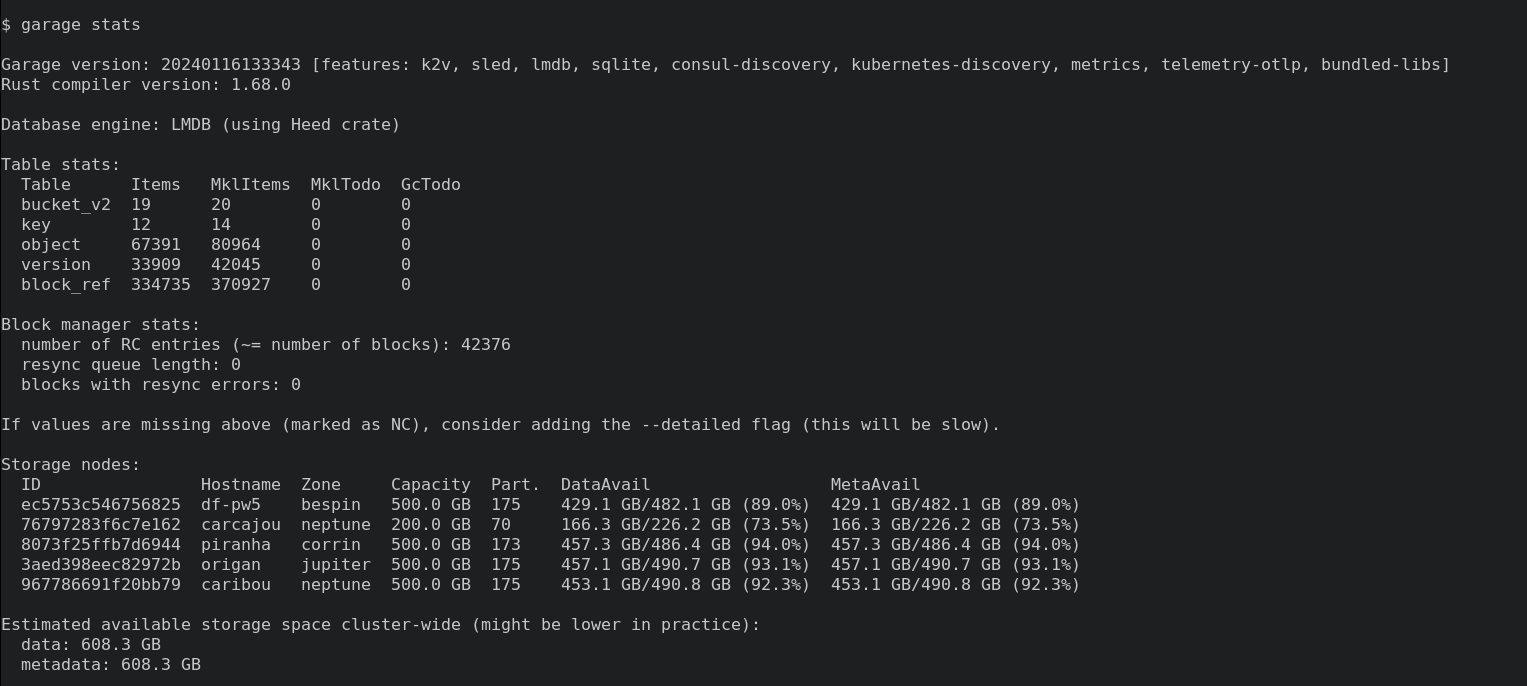
\includegraphics[width=.9\linewidth]{../assets/screenshots/garage_stats_0.10.png}}
		\only<2>{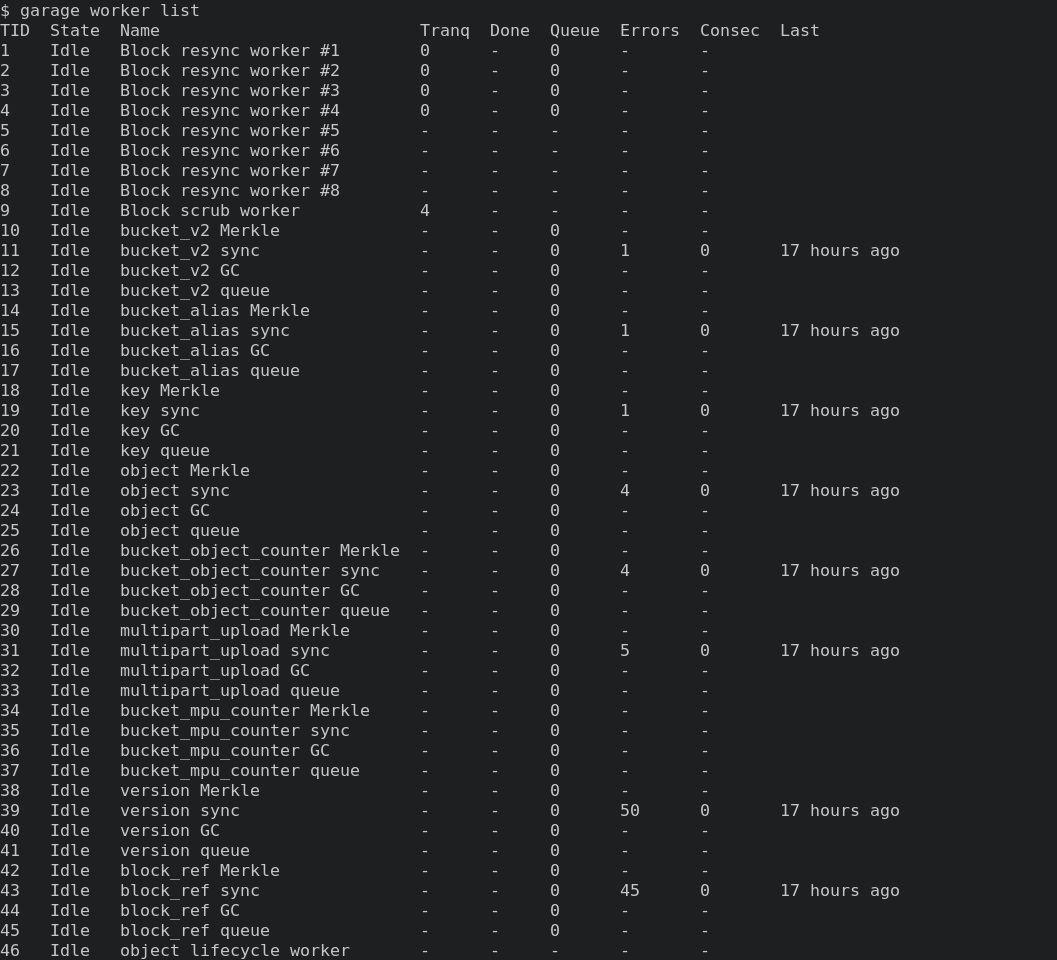
\includegraphics[width=.5\linewidth]{../assets/screenshots/garage_worker_list_0.10.png}}
		\only<3>{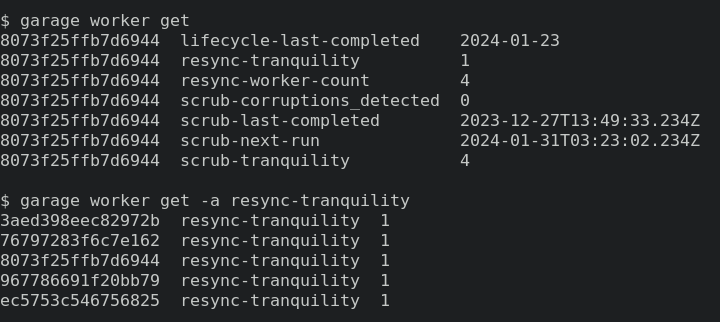
\includegraphics[width=.6\linewidth]{../assets/screenshots/garage_worker_param_0.10.png}}
	\end{center}
\end{frame}

\begin{frame}
	\frametitle{Monitoring with Prometheus + Grafana}
	\begin{center}
		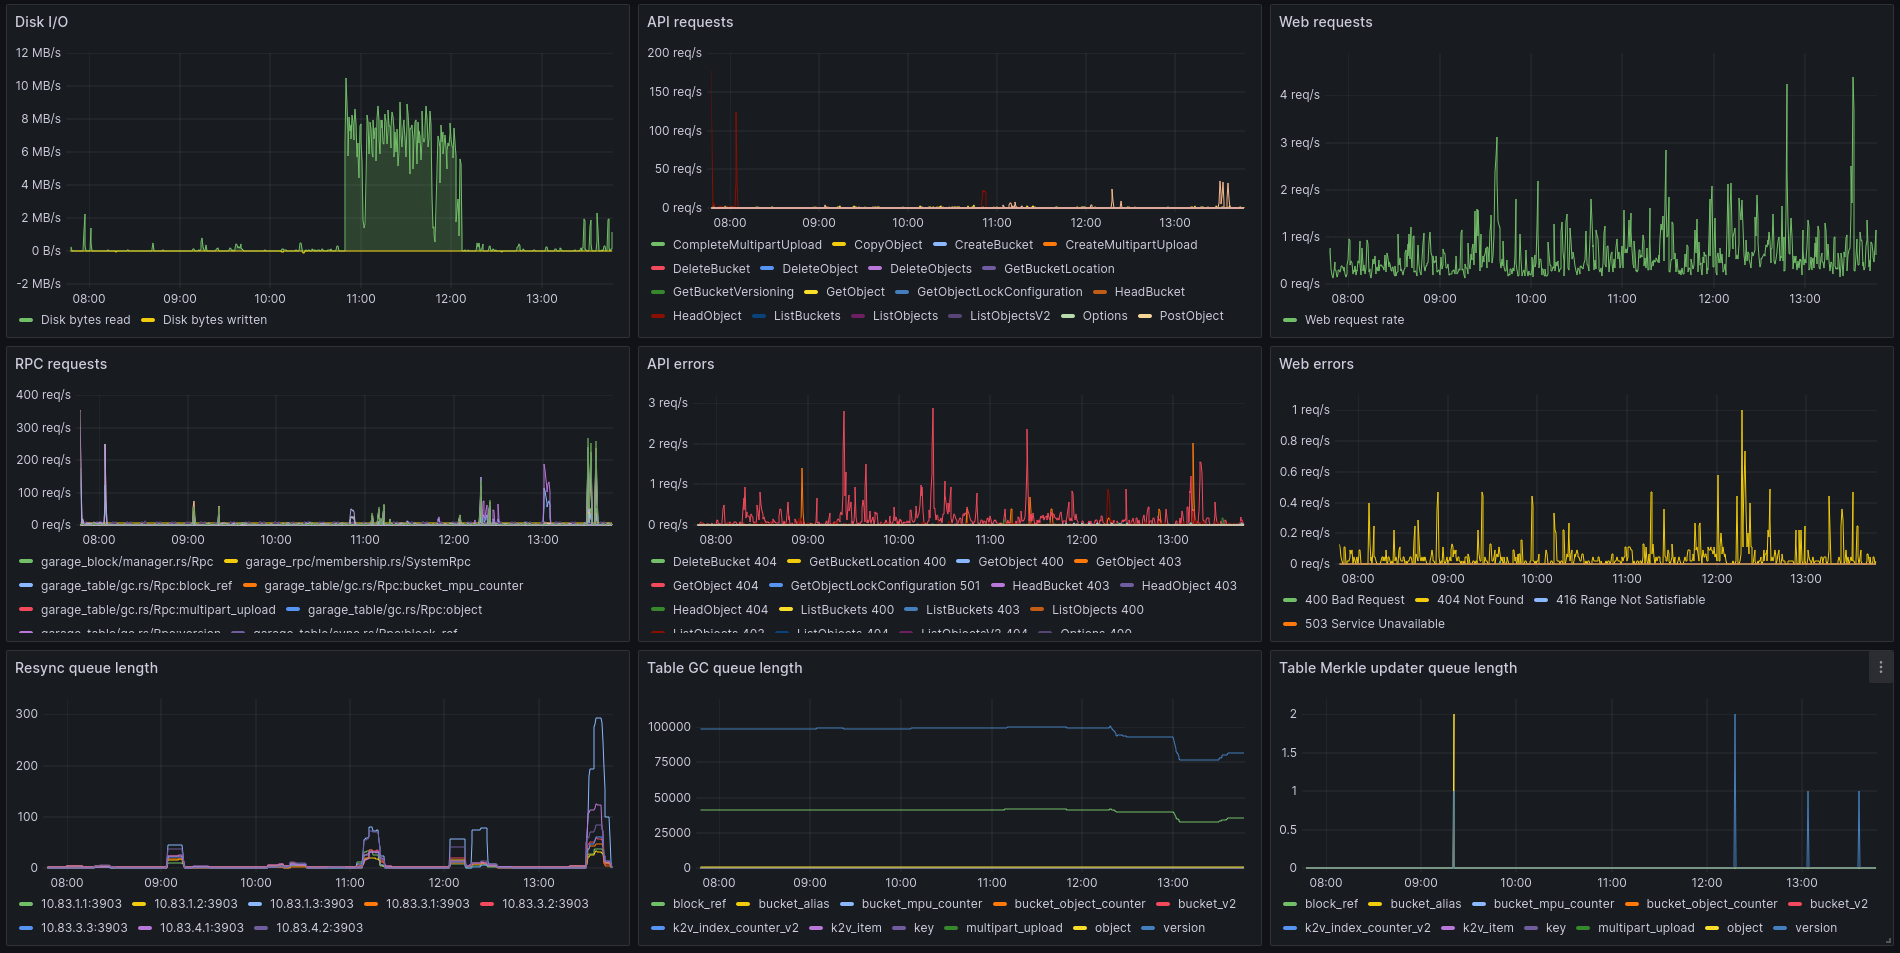
\includegraphics[width=.9\linewidth]{../assets/screenshots/grafana_dashboard.png}
	\end{center}
\end{frame}

\begin{frame}
	\frametitle{Debugging with traces}
	\begin{center}
		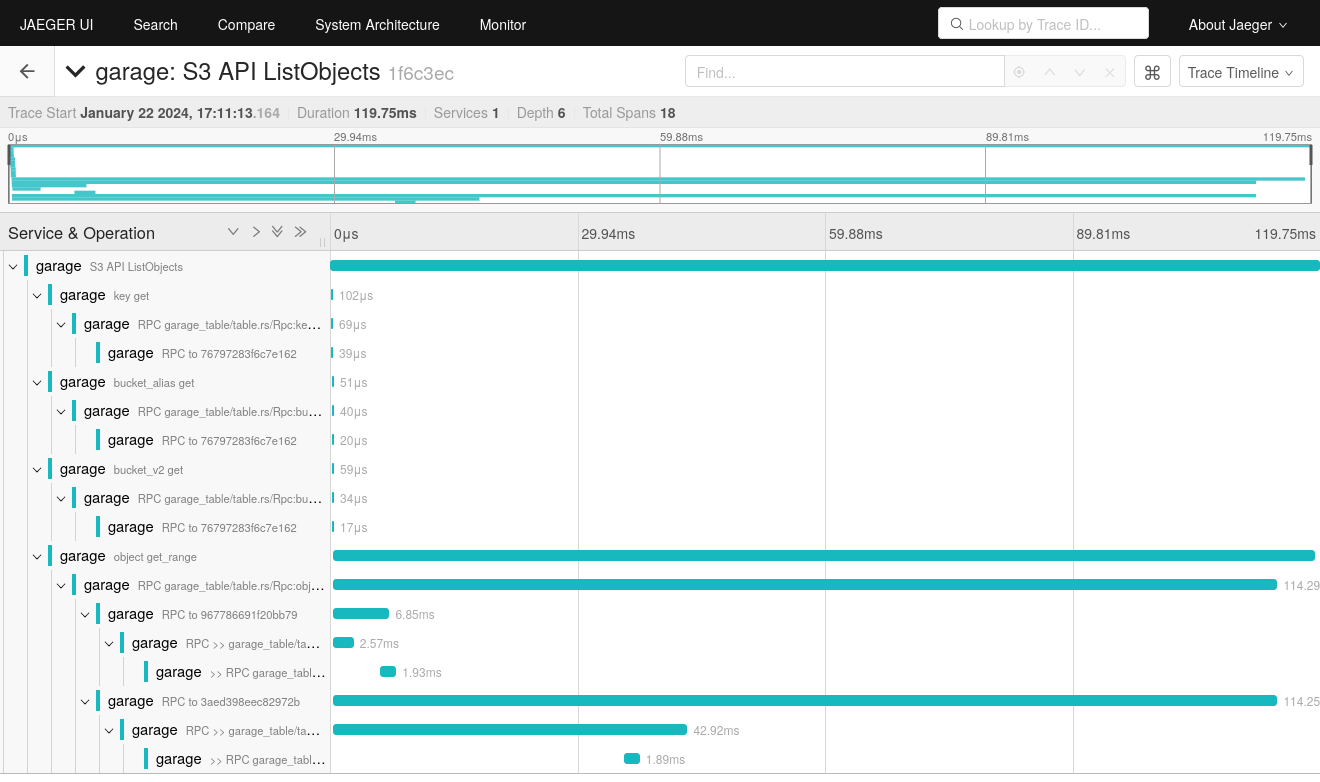
\includegraphics[width=.8\linewidth]{../assets/screenshots/jaeger_listobjects.png}
	\end{center}
\end{frame}

% ---------- SCALING GARAGE ---------

\section{Scaling Garage clusters}

\begin{frame}
	\frametitle{Potential limitations and bottlenecks}
	\begin{itemize}
		\item Global:
			\begin{itemize}
				\item Max. $\sim$100 nodes per cluster (excluding gateways)
			\end{itemize}
			\vspace{1em}
		\item Metadata:
			\begin{itemize}
				\item One big bucket = bottleneck, object list on 3 nodes only
			\end{itemize}
			\vspace{1em}
		\item Block manager:
			\begin{itemize}
				\item Lots of small files on disk
				\item Processing the resync queue can be slow
			\end{itemize}
	\end{itemize}
\end{frame}

\begin{frame}
	\frametitle{Deployment advice for very large clusters}
	\begin{itemize}
		\item Metadata storage:
			\begin{itemize}
				\item ZFS mirror (x2) on fast NVMe
				\item Use LMDB storage engine
			\end{itemize}
			\vspace{.5em}
		\item Data block storage:
			\begin{itemize}
				\item Use Garage's native multi-HDD support
				\item XFS on individual drives
				\item Increase block size (1MB $\to$ 10MB, requires more RAM and good networking)
				\item Tune \texttt{resync-tranquility} and \texttt{resync-worker-count} dynamically
			\end{itemize}
			\vspace{.5em}
		\item Other :
			\begin{itemize}
				\item Split data over several buckets
				\item Use less than 100 storage nodes
				\item Use gateway nodes
			\end{itemize}
			\vspace{.5em}
	\end{itemize}
	Our deployments: $< 10$ TB. Some people have done more!
\end{frame}


% ======================================== END
% ======================================== END
% ======================================== END

\begin{frame}
	\frametitle{Where to find us}
	\begin{center}
			\includegraphics[width=.25\linewidth]{../../logo/garage_hires.png}\\
			\vspace{-1em}
		\url{https://garagehq.deuxfleurs.fr/}\\
		\url{mailto:garagehq@deuxfleurs.fr}\\
		\texttt{\#garage:deuxfleurs.fr} on Matrix

		\vspace{1.5em}
			
\includegraphics[width=.06\linewidth]{../assets/logos/rust_logo.png}
			
\includegraphics[width=.13\linewidth]{../assets/logos/AGPLv3_Logo.png}
	\end{center}
\end{frame}

\end{document}

%% vim: set ts=4 sw=4 tw=0 noet spelllang=en :
